\chapter{Tópicos de gerenciamento de requisitos}

	\section{Rastreabilidade de requisitos}
	Rastrear requisitos é uma atividade que nos permite controlar e visualizar cada parte do processo e garantir que cada parte do desenvolvimento está correto,podemos garantir assim que somente atividades necessárias foram produzidas.

	Rastrear os requisitos através dos estágios de implementação, arquitetura, desing, implementação e teste é importante para garantir a qualidade do software. A habilidade de rastrear os relacionamentos e analisar os impactos causados pelas mudanças é crucial principalmente para atividades que envolvam sistemas críticos. Requisitos que não estão claros podem causar grandes impactos na segurança do projeto e causar um produto não confiável.
	No glossário da IEEE sobre a terminologia da engenharia de software temos a seguinte definição de rastreabilidade:
  	\begin{figure}{!htb}
  		\centering
		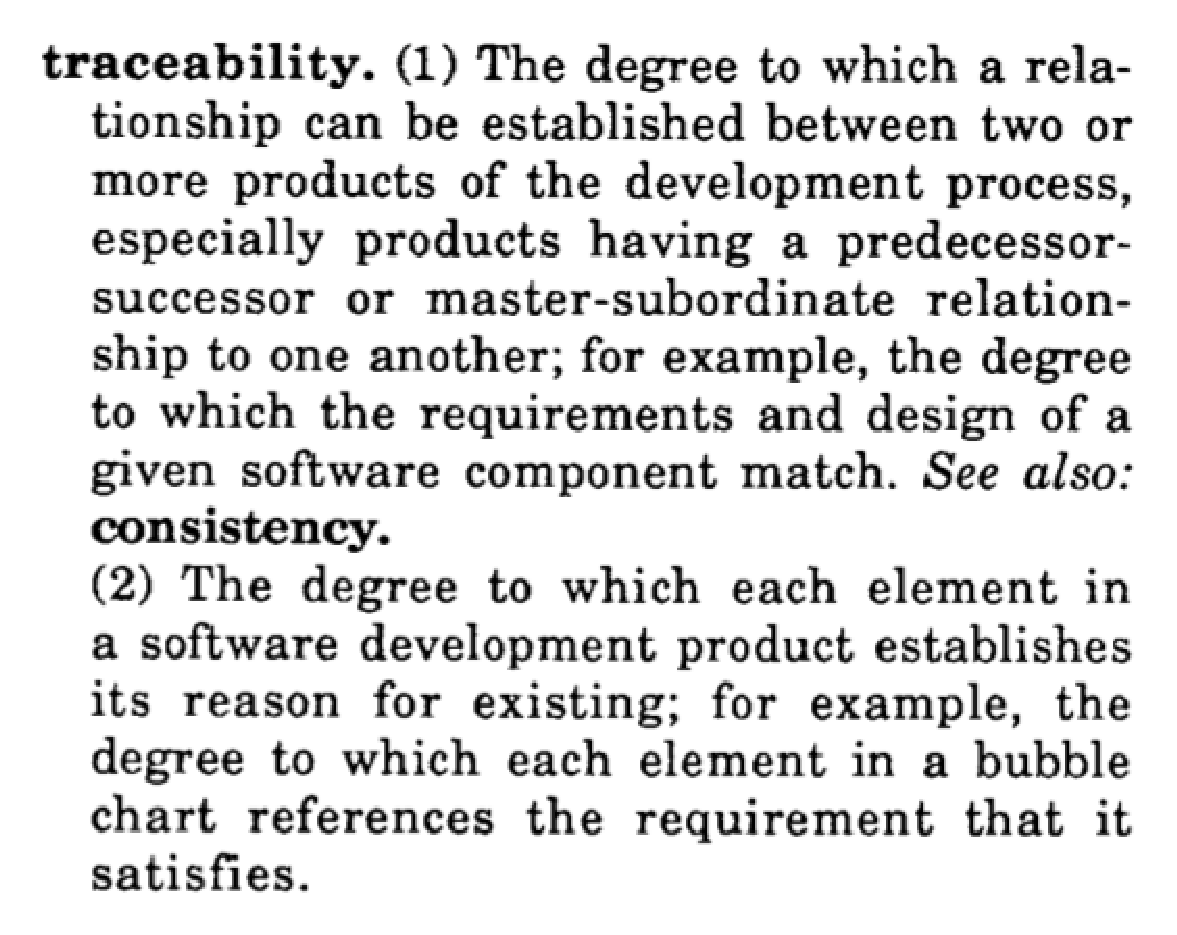
\includegraphics[height=5cm, width=5cm]{figuras/definicao_rastreamento.eps}
		\caption{Definição rastreabilidade IEEE.}
	\end{figure}

	A definição sobre rastreabilidade acima fala sobre a relação do grau de um elemento com o próximo e como cada elemento tem um objetivo bem definido. A rastreabilidade de requisitos pode ser definido então como relação que dois elementos possuem em um mesmo projeto e como estes estão conectados.

	Podemos utilizar várias técnicas para rastrear os requisitos, optamos por usar a rastreabilidade horizontal e vertical, entendemos que elas são claras e diretas, podemos ter uma visão muito boa a partir dessas técnicas.

	\textbf{Rastreabilidade horizontal} - É a rastreabilidade entre diferentes versões ou variações de requisitos, ou outros artefatos, em particular uma fase do ciclo de vida\cite{tese_doutorado}.

	\textbf{Rastreabilidade vertical} - É a rastreabilidade realizada entre requisitos e artefatos produzidos pelo processo de desenvolvimento ao longo do ciclo de vida do projeto.\cite{tese_doutorado}.

	\section{Atributos do requisitos}
	\subsection{Data de criação}
	A data em que o requisito foi criado na ferramenta.
	\subsection{Início planejado}
	Data planejada para o início do desenvolvimento do requisito.
	\subsection{Término planejado}
	Data estipulada para o termino, essa é uma estimativa pode sofrer atrasos.
	\subsection{Data de início}
	Data real em que os responsáveis iniciaram o projeto.
	\subsection{Data de conclusão}
	Data real de término do requisito.
	\subsection{Valor de negócio}
	É a priorização do requisito.
	
	\begin{table}[]
	\centering
	\label{my-label}
		\begin{tabular}{|l|l|}
			\hline
			Prioridade    & Descrição                                                                                                                                        \\ \hline
			Obrigatório   & \begin{tabular}[c]{@{}l@{}}Essencial para o cliente, sem esse requisito as exigência do cliente \\ não são atendidas completamente.\end{tabular} \\ \hline
			Médio         & Requisito importante, mas não impacta nas exigências do cliente.                                                                                 \\ \hline
			Seria bom ter & Útil, porém não agrega valor.                                                                                                                    \\ \hline
		\end{tabular}
	\end{table}

	\subsection{Status}
	Condição atual do requisito. Os Épicos são divididos em  Novo,   Feito   ou   Em   Progresso. Features e Histórias são divididas em Aberta,   Planejada,   Em   Progresso,   Em   Teste   ou   Feita.

	\begin{table}[]
		\centering
		\caption{Épicos}
		\label{my-label}
		\begin{tabular}{|l|l|}
			\hline
			Estado       & Descrição                     \\ \hline
			Novo         & Requisito levantado.          \\ \hline
			Em progresso & Requisito em desenvolvimento. \\ \hline
			Feito        & Concluído.                    \\ \hline
		\end{tabular}
	\end{table}

	\begin{table}[]
		\centering
		\caption{Features e histórias}
		\label{my-label}
		\begin{tabular}{|l|l|}
			\hline
			Estado       & Descrição                     \\ \hline
			Aberto       & Requisito levantado.          \\ \hline
			Planejado    &                               \\ \hline
			Em progresso & Requisito em desenvolvimento. \\ \hline
			Em teste     & Requisito em teste            \\ \hline
			Feito        & Requisito concluído           \\ \hline
			\end{tabular}
	\end{table}

	\subsection{Esforço}
	Uma estimativa feita de dificuldade para implementar um requisito. Uma carta com dificuldade proporcional ao requisito implementado, Planning Poker.
	\begin{figure}{!htb}
  		\centering
		\includegraphics[height=5cm, width=5cm]{figuras/planning_poker.eps}
		\caption{Planning poker}
	\end{figure}
